\documentclass[newpages]{assignment}

\usepackage{booktabs}
\usepackage{float}
\usepackage{tikz}

\class{SI 315}
\title{Assignment 8}
\author{Silas Falde}
\date{Due at 11:59 pm on Wednesday, November 18}
\setcounter{tocdepth}{1}

\begin{document}
\maketitle

\tableofcontents

\section{Basic PageRank}

\begin{problem}
Give an example of a directed connected network with \(n \geq 4\) nodes where not all nodes have the same in-degree (i.e., the network contains two nodes A and B that have different in-degrees) and assigning \(1/n\) to each node is an equilibrium set of Basic PageRank values. Apply the definition of equilibrium to show that assigning \(1/n\) to each node is an equilibrium set of Basic PageRank values.
\end{problem}

\begin{figure}[H]
    \centering
    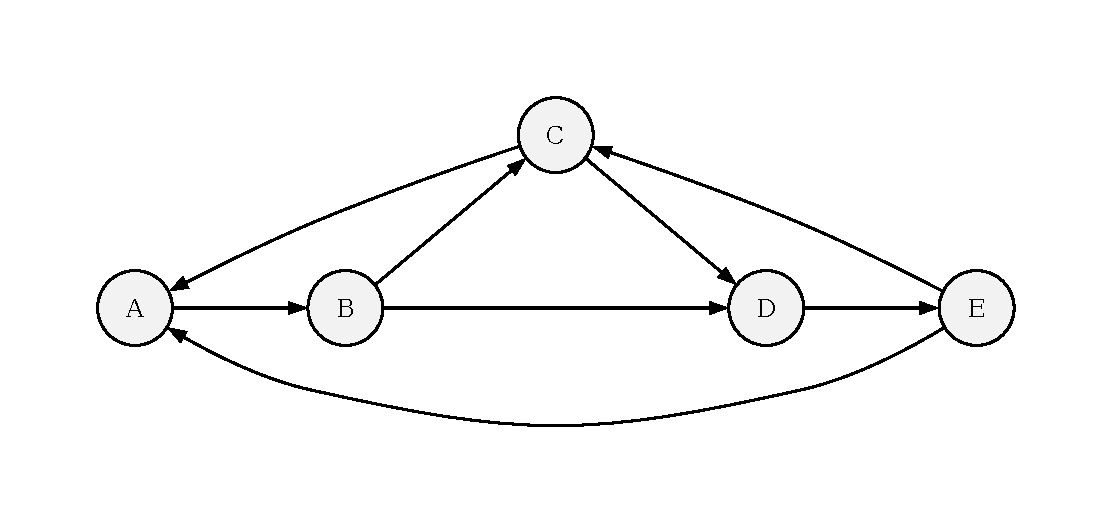
\includegraphics[height=3.5cm]{figures/basic-pagerank-example.pdf}
    \label{fig:hw8-basic-pagerank-example}
    \caption{Example network satisfying the two properties}
\end{figure}
The in-degrees for Figure \ref{fig:hw8-basic-pagerank-example} are \(2,1,2,2,1\) for $A, B, C, D, E$, so they are not all equal.

PageRank updates for each node using $1/5$ as the initial assignment:
\[
    \begin{aligned}
        A & : \frac{1/5}{2}+\frac{1/5}{2}=\frac15, &
        B & : \frac{1/5}{1}=\frac15,                 \\
        C & : \frac{1/5}{2}+\frac{1/5}{2}=\frac15, &
        D & : \frac{1/5}{2}+\frac{1/5}{2}=\frac15, &
        E & : \frac{1/5}{1}=\frac15.
    \end{aligned}
\]
Since one update leaves every value unchanged, assigning \(1/n=1/5\) to each node is an equilibrium.



\section{Scaled PageRank}

\begin{problem}
In class, we discussed what Scaled PageRank is but not how to find it. This question will help you get comfortable doing that. We'll try to calculate a few rounds of the Scaled PageRank values of the following network, with damping parameter \(d=0.8\).
\end{problem}

\begin{figure}[H]
    \centering
    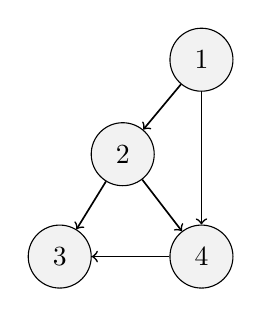
\begin{tikzpicture}[
            node/.style={circle, draw, fill=gray!10, minimum size=0.8cm},
            edge/.style={->, line width=0.6pt}
        ]
        \node[node] (one) at (1, 2) {1};
        \node[node] (two) at (0, 0.8) {2};
        \node[node] (three) at (-0.8, -0.5) {3};
        \node[node] (four) at (1, -0.5) {4};
        \draw[edge] (one) -- (two);
        \draw[edge] (one) -- (four);
        \draw[edge] (two) -- (three);
        \draw[edge] (two) -- (four);
        \draw[edge] (four) -- (three);
    \end{tikzpicture}
    \caption{Network for the Scaled PageRank updates.}
    \label{fig:hw8-pagerank}
\end{figure}

\subsection{}
\begin{problem}
Let's start by getting some intuition about Scaled PageRank. As we discussed in lecture, we can also describe Scaled PageRank values in terms of something called a scaled random walk with damping parameter:

\emph{The walker starts by choosing a page at random, picking each page with equal probability. In each step, the walker does one of two things: With probability \(d\), the walker picks a random outgoing link from their current page, and follows it to where it leads; and with probability \(1-d\) it jumps to a node chosen uniformly at random.}

\begin{enumerate}[label=\roman*.]
    \item Do you expect the Basic PageRank value of node 1 to be larger than zero for large values of \(k\)? Explain your intuition without doing any calculations.
    \item Do you expect the Scaled PageRank value of node 1 to be larger than zero for large values of \(k\) and \(d<1\)? Explain your intuition without doing any calculations.
\end{enumerate}
\end{problem}

Node 1 has no incoming edges, so a basic random walk that follows links cannot reach it after leaving its initial page. Its Basic PageRank becomes zero after the first update and remains zero. With Scaled PageRank, each update gives every node a positive share of the random-jump probability, so node 1 continues to have positive PageRank when $d<1$.

\subsection{}
\begin{problem}
Now we'll calculate Scaled PageRank. Initially, all four nodes have the same Scaled PageRank value of \(1/4\). These are the Scaled PageRank values in round 0. Starting from these values, let's perform the first round of Scaled PageRank updates. We'll talk you through doing this in three steps. Show your work and values for each node after each step.

\begin{enumerate}[label=\roman*.]
    \item Apply the Basic PageRank Update Rule. This step models where the random walker would go if they choose to follow the edges.
    \item Scale down all PageRank values by a factor of \(d\). That is, multiply each node's value from (i) by \(d=0.8\). This step models the fact that, in Scaled PageRank, the random walker only follows the edges with probability \(d\) (and chooses to jump randomly the rest of the time).
    \item Divide the residual \(1-d\) units of PageRank equally over all nodes, giving \((1-d)/n\) to each. That is, add \((1-d)/n=0.2/4=0.05\) to each node's value from (ii). This step models the fact that every node has an equal chance of being visited by the random walker when it chooses to jump randomly.
\end{enumerate}
\end{problem}

\[
\begin{aligned}
P_1(1)&=0, &
P_1(2)&=\frac{1/4}{2}=\frac18, &
P_1(3)&=\frac{1/4}{2}+\frac{1/4}{1}=\frac38, &
P_1(4)&=\frac{1/4}{2}+\frac{1/4}{2}=\frac14.
\end{aligned}
\]
Scaling these values by $0.8$ and adding $0.05$ to each gives:
\begin{center}
    \begin{tabular}{ccccc}
        \toprule
        Step & Node 1 & Node 2 & Node 3 & Node 4 \\
        \midrule
        Basic update & $0$ & $1/8$ & $3/8$ & $1/4$ \\
        Multiply by $0.8$ & $0$ & $1/10$ & $3/10$ & $1/5$ \\
        Add $0.05$ & $1/20$ & $3/20$ & $7/20$ & $1/4$ \\
        \bottomrule
    \end{tabular}
\end{center}
Thus the round-1 Scaled PageRank values are $(1/20,3/20,7/20,1/4)$ for nodes $1$ through $4$.

\subsection{}
\begin{problem}
Now perform a second round of Scaled PageRank updates, using the steps from part c. Show your work and values for each node after each step.
\end{problem}

\[
\begin{aligned}
P_2(1)&=0, &
P_2(2)&=\frac{1/20}{2}=\frac1{40}, &
P_2(3)&=\frac{3/20}{2}+\frac14=\frac{13}{40}, &
P_2(4)&=\frac{1/20}{2}+\frac{3/20}{2}=\frac1{10}.
\end{aligned}
\]
After scaling and adding the random-jump share:
\begin{center}
    \begin{tabular}{ccccc}
        \toprule
        Step & Node 1 & Node 2 & Node 3 & Node 4 \\
        \midrule
        Basic update & $0$ & $1/40$ & $13/40$ & $1/10$ \\
        Multiply by $0.8$ & $0$ & $1/50$ & $13/50$ & $2/25$ \\
        Add $0.05$ & $1/20$ & $7/100$ & $31/100$ & $13/100$ \\
        \bottomrule
    \end{tabular}
\end{center}
The round-2 values are $(1/20,7/100,31/100,13/100)$.

\subsection{}
\begin{problem}
Find an equilibrium set of Basic PageRank values for this graph. Explain why these values are an equilibrium set.

\textit{Hint:} You should be able to find the values using intuition (which you don't need to explain) and then explain why that set of values is an equilibrium set.
\end{problem}

\[
x_1=0,\qquad
x_2=\frac{x_1}{2},\qquad
x_3=\frac{x_2}{2}+x_4,\qquad
x_4=\frac{x_1}{2}+\frac{x_2}{2}.
\]
The first equation forces $x_1=0$, then $x_2=0$ and $x_4=0$, and finally $x_3=0$. Therefore $(0,0,0,0)$ is an equilibrium: applying one Basic PageRank update leaves all four values unchanged. Node 3 has no outgoing links, so under the stated Basic PageRank rule its value is not passed to another node.

\subsection{}
\begin{problem}
Find an equilibrium set of Scaled PageRank values with damping parameter \(d=0.8\) for this graph. Explain why these values are an equilibrium set.

\textit{Hint:} One way to find this equilibrium set of values is to go through the following four steps:
\begin{enumerate}[label=(\roman*)]
    \item Let \(x_1\) be the equilibrium value of node 1. Write out the equation that \(x_1\) must satisfy. What must \(x_1\) be equal to?
    \item Let \(x_2\) be the equilibrium value of node 2. Write out the equation that \(x_2\) must satisfy. Given your answer to (i), what must \(x_2\) be equal to?
    \item Let \(x_4\) be the equilibrium value of node 4. Write out the equation that \(x_4\) must satisfy. Given your answer to (i) and (ii), what must \(x_4\) be equal to?
    \item What is the equilibrium value of node 3? Explain.
\end{enumerate}
\end{problem}

Using the Scaled PageRank update rule with $d=0.8$, each equilibrium value satisfies
\[
\begin{aligned}
x_1&=0.8(0)+0.05=0.05=\frac1{20},\\
x_2&=0.8\left(\frac{x_1}{2}\right)+0.05
    =0.8\left(\frac1{40}\right)+0.05=0.07=\frac7{100},\\
x_4&=0.8\left(\frac{x_1}{2}+\frac{x_2}{2}\right)+0.05
    =0.8\left(\frac1{40}+\frac7{200}\right)+0.05=0.098=\frac{49}{500},\\
x_3&=0.8\left(\frac{x_2}{2}+x_4\right)+0.05
    =0.8\left(\frac7{200}+\frac{49}{500}\right)+0.05=0.1564=\frac{391}{2500}.
\end{aligned}
\]
The equations successively determine nodes 1, 2, and 4, and then node 3. Substituting these values into the update rule reproduces each value, so $(x_1,x_2,x_3,x_4)=(1/20,7/100,391/2500,49/500)$ is an equilibrium. The total is less than $1$ because node 3 has no outgoing links and the class update rule does not redistribute its rank.

\section{VCG Advertising Auction}

\begin{problem}
A search engine has three advertising slots available for sale. Three advertisers, A, B, and C, are interested in these slots. The click-through rates and the advertisers' true values per click are shown below.

\begin{center}
    \begin{tabular}{cccc}
        \toprule
        Slot & Click-through rate & Advertiser & Value per click \\
        \midrule
        X    & 10                 & A          & \$10            \\
        Y    & 5                  & B          & \$8             \\
        Z    & 0                  & C          & \$4             \\
        \bottomrule
    \end{tabular}
\end{center}

The search engine uses the VCG procedure to assign advertising slots and determine prices. Show your work for each calculation.
\end{problem}

\subsection{}
\begin{problem}
Assuming all advertisers bid their true values, calculate the valuations of each advertiser for all three slots. Find the socially optimal assignment.
\end{problem}

\begin{center}
    \begin{tabular}{lrrr}
        \toprule
        & Slot X (10 clicks) & Slot Y (5 clicks) & Slot Z (0 clicks) \\
        \midrule
        A ($\$10$/click) & \$100 & \$50 & \$0 \\
        B ($\$8$/click)  & \$80 & \$40 & \$0 \\
        C ($\$4$/click)  & \$40 & \$20 & \$0 \\
        \bottomrule
    \end{tabular}
\end{center}
The socially optimal assignment is A to X, B to Y, and C to Z, with total valuation $100+40+0=\$140$.

\subsection{}
\begin{problem}
Calculate the VCG price and payoff for each advertiser under this assignment. Show how you calculate the harm done to the other advertisers.
\end{problem}

\begin{center}
    \begin{tabular}{lrrr}
        \toprule
        Advertiser & Others' value without advertiser & Others' value in assignment & VCG price \\
        \midrule
        A & $80+20=100$ & $40+0=40$ & \$60 \\
        B & $100+20=120$ & $100+0=100$ & \$20 \\
        C & $100+40=140$ & $100+40=140$ & \$0 \\
        \bottomrule
    \end{tabular}
\end{center}
An advertiser's VCG price is the other advertisers' best total valuation without that advertiser, minus their total valuation in the chosen assignment. For example, without A, B gets X and C gets Y, giving the other advertisers \$100; with A present, their assigned value is \$40. The resulting payoffs (true value minus VCG price) are A: $100-60=\$40$, B: $40-20=\$20$, and C: $0-0=\$0$.

\subsection{}
\begin{problem}
Suppose Advertisers A and B agree that A will continue bidding \$10 per click, while B will lower their bid from \$8 to \$5 per click. Advertiser C continues bidding \$4 per click. Using these bids, find the new assignment and VCG prices. Then calculate A's and B's payoffs using their true values per click.
\end{problem}

Using the reported bids, the valuations are A: $(100,50,0)$, B: $(50,25,0)$, and C: $(40,20,0)$ for slots X, Y, and Z, respectively. The maximizing assignment remains A to X, B to Y, and C to Z, with reported total value \$125. The VCG prices are:
\[
\begin{aligned}
p_A&=(50+20)-25=\$45,\\
p_B&=(100+20)-100=\$20,\\
p_C&=0.
\end{aligned}
\]
The prices use reported values to find the assignment and harm. Payoffs use the advertisers' true values: A receives $100-45=\$55$, and B receives $40-20=\$20$.

\subsection{}
\begin{problem}
Compare the combined payoffs of A and B in parts (b) and (c). Does either advertiser benefit from the change in bids? Does this contradict the result that truthful bidding is a dominant strategy in the VCG procedure? Explain briefly.
\end{problem}

With truthful bids, A and B's combined payoff is $40+20=\$60$; with B's lower bid, it is $55+20=\$75$. A benefits from B's misreport, while B's payoff is unchanged. This does not contradict the dominant-strategy result: it concerns one advertiser changing their own bid while the other bids are held fixed. Here A and B change bids as a group, so A can benefit from B's coordinated misreport.

\section{VCG Auction Prices}

\begin{problem}
Consider the following VCG auction and prices. In this problem, we'll walk you through a few steps to find the values of \(x\), \(y\), and \(z\).
\end{problem}

\begin{figure}[H]
    \centering
    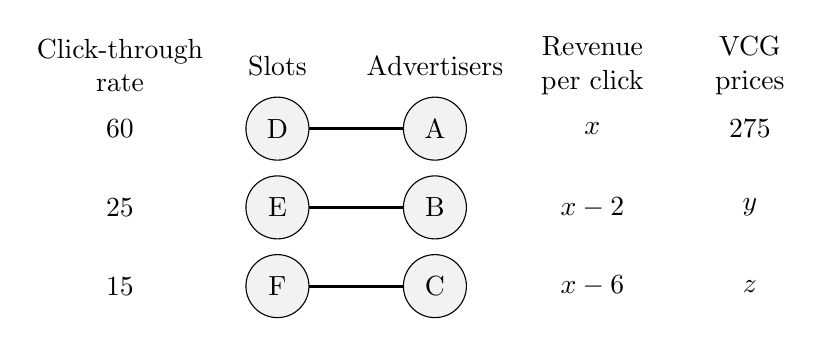
\begin{tikzpicture}[
            buyer/.style={circle, draw, fill=gray!10, minimum size=0.8cm},
            edge/.style={line width=1pt}
        ]
        \node[align=center] at (-2, 0.8) {Click-through\\rate};
        \node at (0, 0.8) {Slots};
        \node at (2, 0.8) {Advertisers};
        \node[align=center] at (4, 0.8) {Revenue\\per click};
        \node[align=center] at (6, 0.8) {VCG\\prices};
        \node[buyer] (D) at (0, 0) {D};
        \node[buyer] (E) at (0, -1) {E};
        \node[buyer] (F) at (0, -2) {F};
        \node[buyer] (A) at (2, 0) {A};
        \node[buyer] (B) at (2, -1) {B};
        \node[buyer] (C) at (2, -2) {C};
        \draw[edge] (D) -- (A);
        \draw[edge] (E) -- (B);
        \draw[edge] (F) -- (C);
        \node at (-2, 0) {60};
        \node at (-2, -1) {25};
        \node at (-2, -2) {15};
        \node at (4, 0) {\(x\)};
        \node at (4, -1) {\(x-2\)};
        \node at (4, -2) {\(x-6\)};
        \node at (6, 0) {275};
        \node at (6, -1) {\(y\)};
        \node at (6, -2) {\(z\)};
    \end{tikzpicture}
    \caption{VCG auction values and prices.}
    \label{fig:hw8-vcg}
\end{figure}

\subsection{}
\begin{problem}
List the valuations for each buyer in terms of \(x\).
\end{problem}

\begin{center}
    \begin{tabular}{lccc}
        \toprule
        & Slot D (60 clicks) & Slot E (25 clicks) & Slot F (15 clicks) \\
        \midrule
        A & $60x$ & $25x$ & $15x$ \\
        B & $60(x-2)$ & $25(x-2)$ & $15(x-2)$ \\
        C & $60(x-6)$ & $25(x-6)$ & $15(x-6)$ \\
        \bottomrule
    \end{tabular}
\end{center}
Each entry is the slot's click-through rate times that buyer's revenue per click.

\subsection{}
\begin{problem}
Calculate the VCG price of D in terms of \(x\), then find the value of \(x\) such that the VCG price of D is 275. Show your work.
\end{problem}

\[
\begin{aligned}
p_D
&=\bigl[60(x-2)+25(x-6)\bigr]
 -\bigl[25(x-2)+15(x-6)\bigr]\\
&=45x-130.
\end{aligned}
\]
Without A, B takes D and C takes E; in the displayed assignment, B takes E and C takes F. Setting the harm to the specified VCG price gives $45x-130=275$, so $x=9$.

\subsection{}
\begin{problem}
Plug in the value of \(x\) from part (b) into the market. What values do \(y\) and \(z\) have to be, at this value of \(x\)? Show your work.
\end{problem}

At $x=9$, the per-click values are A: \$9, B: \$7, and C: \$3, so the displayed assignment is optimal. Without B, C moves from F to E while A remains in D, making the harm to the other advertisers $25(3)-15(3)=\$30$; hence $y=30$. Without C, A and B remain in D and E, so C causes no harm and $z=0$.

\section{VCG and GSP Auctions}

\begin{problem}
Suppose a search engine has three ad slots to sell. Slot A has a clickthrough rate of 10, slot B has a clickthrough rate of 8, and slot C has a clickthrough rate of 3. There are four advertisers who are interested in these slots. Advertiser W values clicks at \$11 per click, Advertiser X values clicks at \$7 per click, advertiser Y values clicks at \$3 per click, and advertiser Z values clicks at \$1 per click.
\end{problem}

\subsection{}
\begin{problem}
Assuming each advertiser bids their true value, compute the socially optimal allocation of slots to advertisers and the VCG price for each slot. Show all your work.
\end{problem}

\begin{center}
    \begin{tabular}{lrrr}
        \toprule
        & Slot A (10 clicks) & Slot B (8 clicks) & Slot C (3 clicks) \\
        \midrule
        W (\$11/click) & \$110 & \$88 & \$33 \\
        X (\$7/click)  & \$70 & \$56 & \$21 \\
        Y (\$3/click)  & \$30 & \$24 & \$9 \\
        Z (\$1/click)  & \$10 & \$8 & \$3 \\
        \bottomrule
    \end{tabular}
\end{center}
The socially optimal allocation is W to A, X to B, and Y to C; Z is unassigned. The VCG payment is the harm to the other advertisers:
\[
\begin{aligned}
p_W&=(70+24+3)-(56+9)=\$32,\\
p_X&=(110+24+3)-(110+9)=\$18,\\
p_Y&=(110+56+3)-(110+56)=\$3.
\end{aligned}
\]
These are total payments. Dividing by the allocated click-through rates, the corresponding per-click prices are \$3.20 for W, \$2.25 for X, and \$1 for Y.

\subsection{}
\begin{problem}
Assuming each advertiser bids their true value, compute the socially optimal allocation of slots to advertisers and the GSP price for each slot. Show all your work.
\end{problem}

\begin{center}
    \begin{tabular}{lccc}
        \toprule
        Advertiser & Slot & GSP price per click & Total payment \\
        \midrule
        W & A & \$7 & $10(7)=\$70$ \\
        X & B & \$3 & $8(3)=\$24$ \\
        Y & C & \$1 & $3(1)=\$3$ \\
        \bottomrule
    \end{tabular}
\end{center}
The truthful-bid ranking is W, X, Y, Z, and each slot is priced at the next-highest bid per click.

\subsection{}
\begin{problem}
Suppose advertiser W lowers their bid to \$6, while the other advertisers continue bidding their true values. Under GSP, what slot will W receive? Calculate W's payoff before and after lowering their bid. Would W benefit from this change? What does this imply about truthful bidding under GSP compared with VCG?
\end{problem}

After lowering the bid, the ranking is X, W, Y, Z, so W receives slot B and pays Y's \$3 bid per click. Before lowering the bid, W's payoff was $10(11-7)=\$40$. After lowering it, W's payoff is $8(11-3)=\$64$, so W benefits by \$24. This illustrates that truthful bidding need not be a dominant strategy in GSP, unlike in VCG.

\end{document}